\section{Monte Carlo datasets}
For this analysis two MC productions have been used, both anchored to the 2010 pp data taking periods (LHC10b, LHC10c, LHC10d, LHC10e).
Both simulations use PYTHIA6 with the Perugia2011 tune as particle generator with $\s=7$~TeV.

The production tagged LHC14j4b, LHC14j4c, LHC14j4d, LHC14j4e is a minimum-bias production with roughly the same statistics as the one collected in real data-taking.
This production has been used to test the analysis techniques, in particular to validate the ability of the analysis chain to recover the yield of the signal.

The production tagged LHC15i2b, LHC15i2c, LHC15i2d, LHC15i2e is a production binned in $p_{\rm T,hard}$ bins.
In addition the charm content has been enhanced by requesting a \ccbar\ in 50\% of the events and a \bbbar\ in the remaining half.

Results shown below come from the LEGO train Jets\_EMC\_pp\_MC, run n. 949 (LHC15i2b), 950 (LHC15i2c), 951 (LHC15i2d), 952 (LHC15i2e), 953 (LHC14j4b), 954 (LHC14j4c), 955 (LHC14j4d), 956 (LHC14j4e).
\section{Overview of the analysis}
The \Dzero\ meson candidates are selected using the ``standard 2010 pp'' cuts, which are accessed through the static method AliRDHFCuts::SetStandardCutsPP2010().

For each \Dzero\ candidate a separate jet finding is performed. The daughters of the \Dzero\ candidate are 
removed from the collection of hybrid tracks; the 4-momentum of the \Dzero\ candidate is added back. 
This collection of tracks plus \Dzero\ candidate is used as input for the jet finder.
The jet finder algorithm is \antikt\ with a resolution parameter $R=0.4$ in its FastJet (v. 3.1.3) implementation.

For the estimation of the detector resolution and reconstruction efficiency, only real \Dzero\ coming from
the fragmentation of a charm quark are considered. \Dzero\ candidates are matched with generator-level \Dzero\ using their MC label.

The main analysis tasks (C++ classes) used in the analysis are in the PWGJE library:
\begin{itemize}
\item AliAnalysisTaskDmesonJets
\item AliAnalysisTaskDmesonJetsDetectorResponse
\end{itemize}
%%%%%%%%%%%%
%%%%%%%%%%%%
\section{Simulation figures}
%%%%%%%%%%%%
In the following paragraphs the figures prepared for the Hot Quarks 2016 conference are presented.
%%%%
\subsection{Jet momentum resolution and reconstruction efficiency}
%%%%
Figure~\ref{fig:HQ16_Simulation_EfficiencyVsDPt} shows the jet reconstruction efficiency as a function of \ptd\ in 4 different \ptchjet\ bins.
It is noteworthy that the efficiency does not show any observable dependence on \ptchjet.
The efficiency is taken as the ratio of the \ptd\ spectra of the D-tagged particle-level jets for which a matched
D-tagged detector-level jet was found overall the D-tagged particle-level jets (regardless of whether they are matched to a detector-level jet).
For the detector-level jets, the D meson is required to be within the standard fiducial rapidity cuts implemented in the AliRDHFCutsD0toKpi class.
Jets are further requested to have $|\eta_{\rm jet}| < 0.9 - R$, both at particle and detector levels.
\begin{figure}[tbh]
\begin{center}
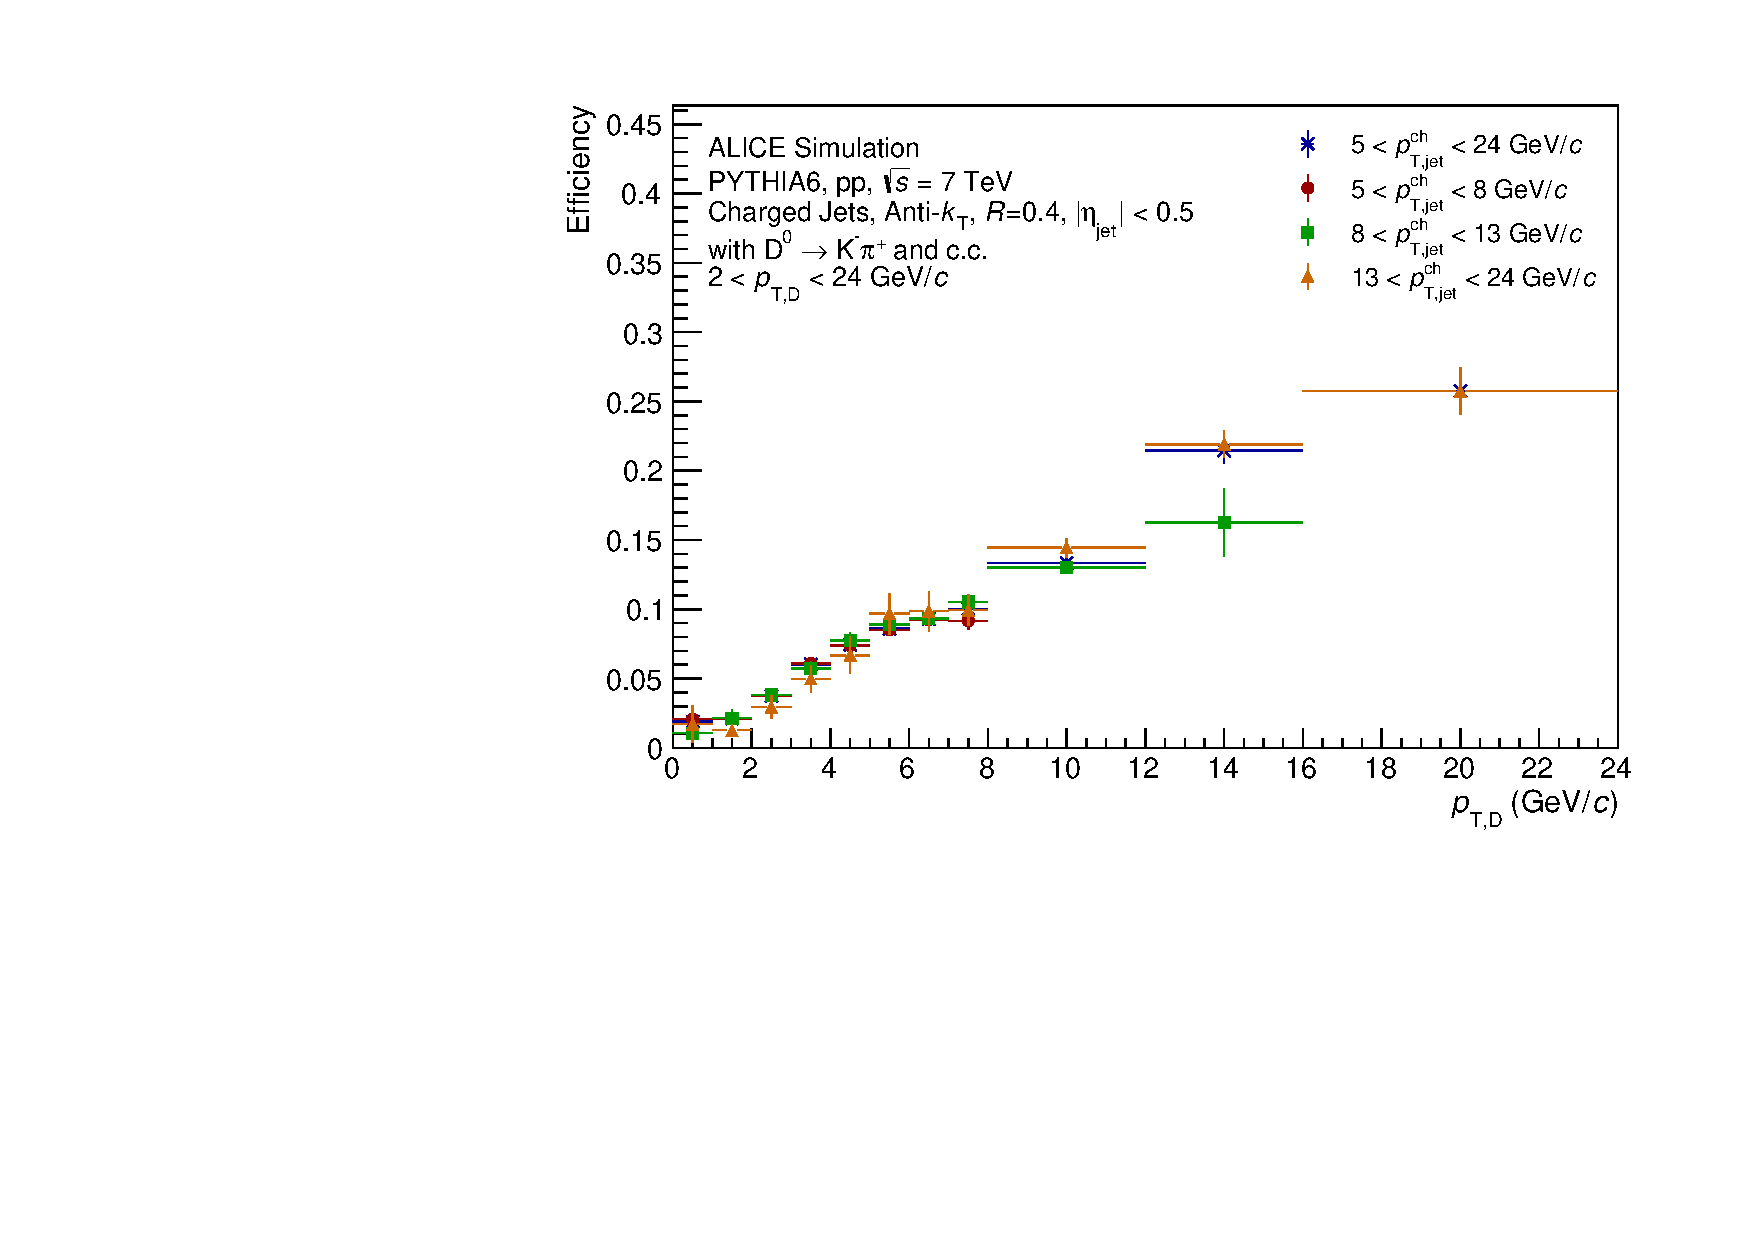
\includegraphics[width=0.8\textwidth]{img/HQ16_Simulation_EfficiencyVsDPt}
 \caption{Jet reconstruction efficiency as a function of \ptd\ in \ptchjet\ bins.} 
 \label{fig:HQ16_Simulation_EfficiencyVsDPt}
\end{center}
\end{figure}

The jet momentum resolution and energy scale shift are estimated calculating the variable:
\begin{equation}
(p_{\mathrm{T,ch jet}}^{\mathrm{det}} - p_{\mathrm{T,ch jet}}^{\mathrm{part}}) / p_{\mathrm{T,ch jet}}^{\mathrm{part}}
\label{eq:detResp}
\end{equation}
for each matched pair of a particle-level jet with a detector-level jet.
Figure~\ref{fig:HQ16_Simulation_DetectorResponse} shows the probability density distribution of Eq.~\ref{eq:detResp}.
The median and the mean of these distributions are shown as a function of \ptchjetgen\ in Fig.~\ref{fig:HQ16_Simulation_EnergyScaleShift}.
This gives an estimate of the relative energy scale shift that needs to be corrected for.
The jet momentum resolution is estimated looking at the standard deviation of the distribution of Eq.~\ref{eq:detResp} as a function
of \ptchjetgen, shown in Fig.~\ref{fig:HQ16_Simulation_Resolution}.
\begin{figure}[tbh]
\centering
\begin{subfigure}[b]{0.49\textwidth}
  \centering
  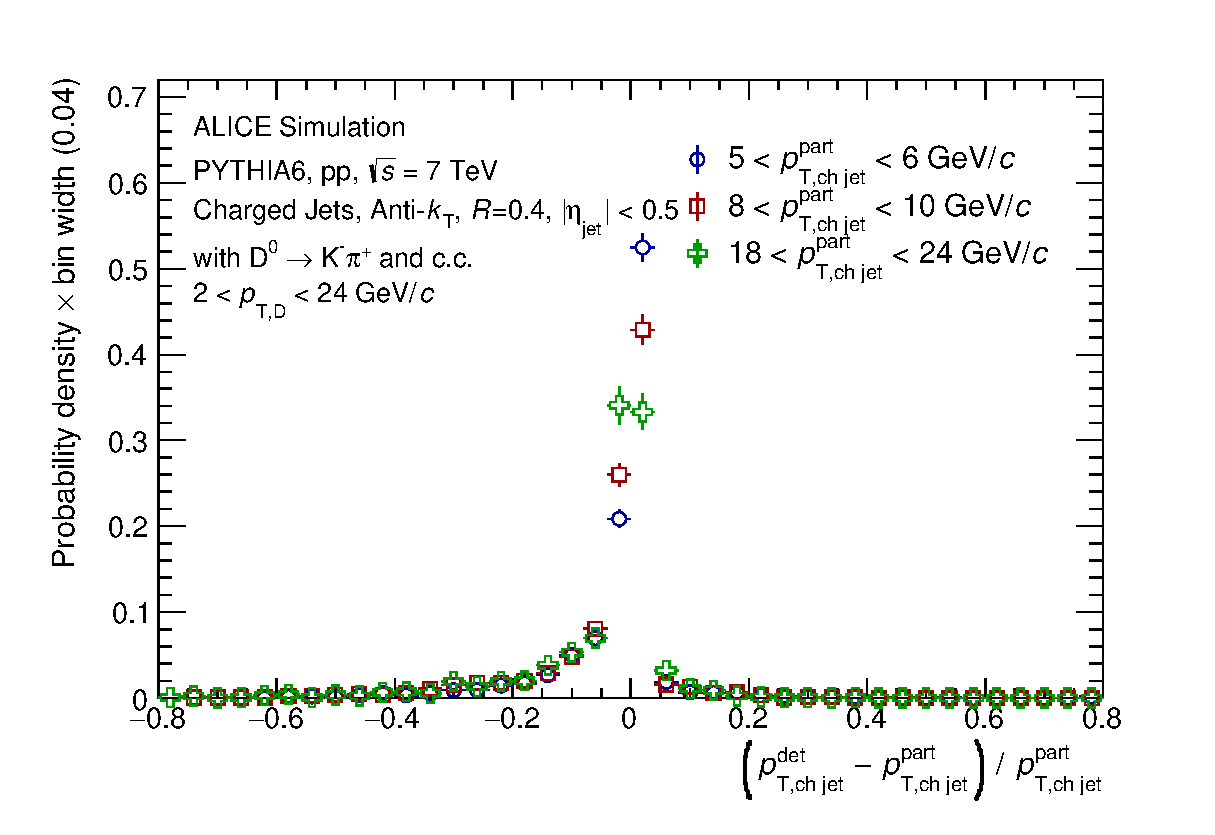
\includegraphics[width=1.0\linewidth]{img/HQ16_Simulation_DetectorResponse}
  \caption{Probability density distribution}
  \label{fig:HQ16_Simulation_DetectorResponse}
\end{subfigure}\\
\begin{subfigure}{0.49\textwidth}
  \centering
  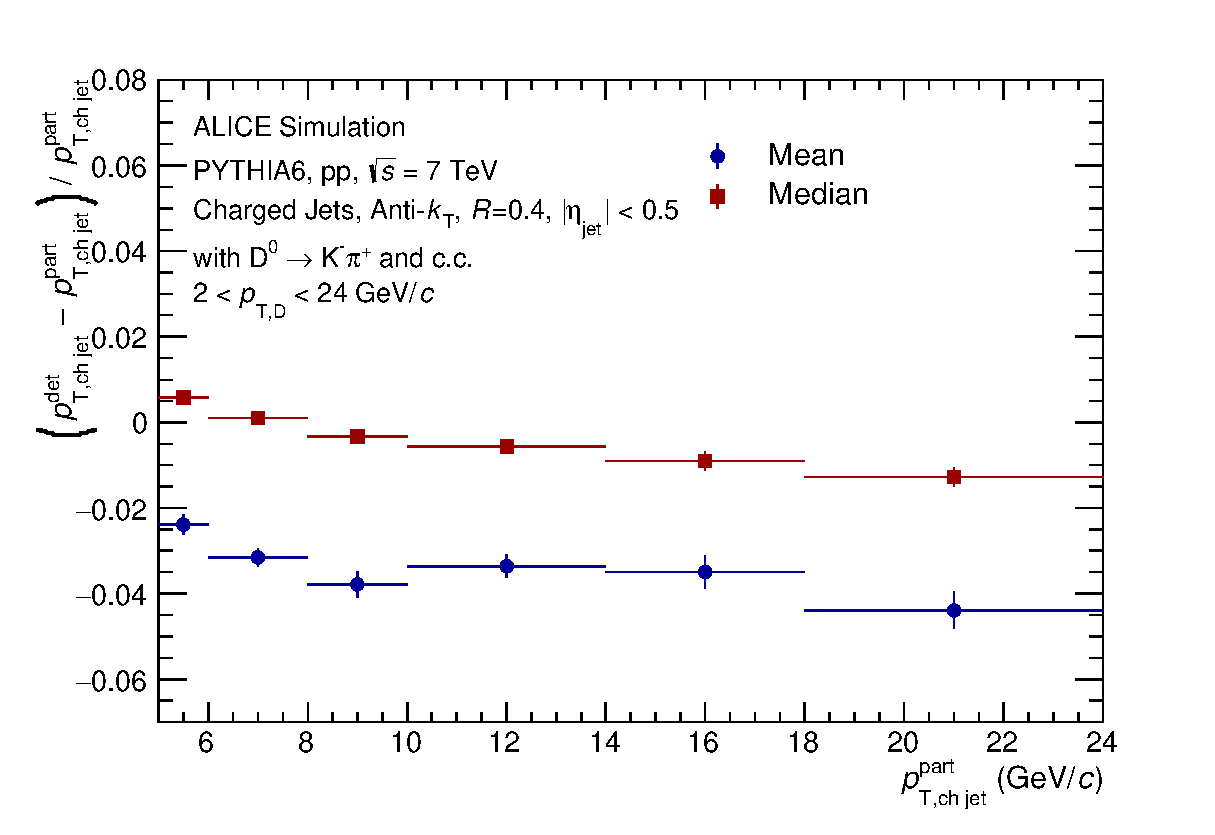
\includegraphics[width=1.0\linewidth]{img/HQ16_Simulation_EnergyScaleShift}
  \caption{Energy scale shift}
  \label{fig:HQ16_Simulation_EnergyScaleShift}
\end{subfigure}
\begin{subfigure}{0.49\textwidth}
  \centering
  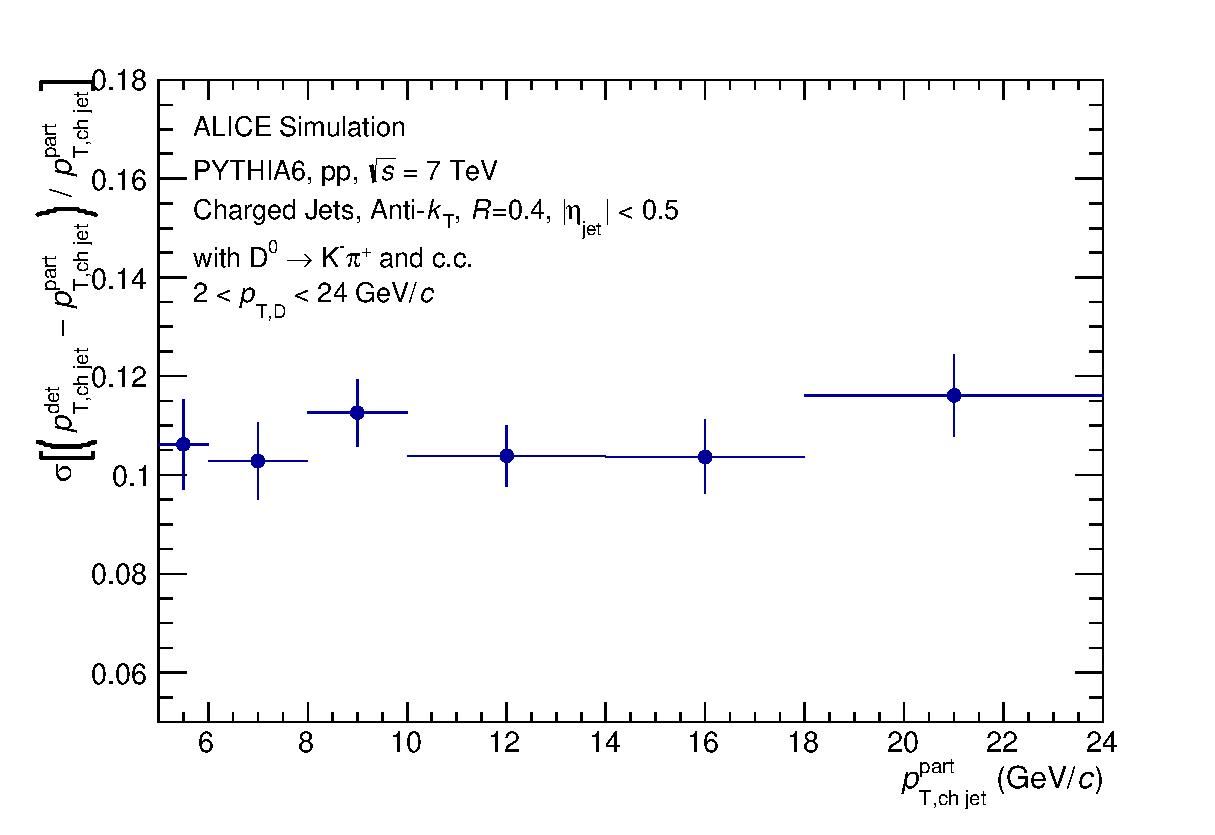
\includegraphics[width=1.0\linewidth]{img/HQ16_Simulation_Resolution}
  \caption{Resolution}
  \label{fig:HQ16_Simulation_Resolution}
\end{subfigure}
\caption{The variable (\ptchjetdet $-$ \ptchjetgen) / \ptchjetgen\ is used to estimate the corrections that need to be applied for the detector effects.}
\label{fig:DetectorResponse}
\end{figure}
%%%%
\subsection{Signal extraction}
%%%%
Three methods for the signal extraction have been implemented and tested in MC.
In the first method the \Dzero\ meson candidates are divided in bins of jet \pt. The invariant mass distributions
are fit using a Gaussian for the signal and an exponential function for the background.
For the second and third methods the \Dzero\ candidates are divided in bins of \ptd. 
The invariant mass distributions in bins of \ptd\ are fit with the same function as above. The
peak position and its width are estimated from the fit, as well as the amount of background in the peak region ($|M_{\mathrm{K\pi}}-M_{\mathrm{fit}}) < 2\sigma_{\mathrm{fit}}$).
Then for each \ptd\ bin the \ptchjet\ distribution of the \Dzero\ candidates is extracted.
For the side-band (S-B) method the background is estimated from the \ptchjet\ distribution of the \Dzero\ candidates in the side bands ($4\sigma_{\mathrm{fit}} < |M_{\mathrm{K\pi}}-m_{\mathrm{fit}}) < 8\sigma_{\mathrm{fit}}$).
For the like-sign (L-S) method the background is estimated from the \ptchjet\ distribution of the like-sign pairs in the \Dzero\ peak region.
In both cases, the background \ptchjet\ distributions are normalized using the total background estimated from the invariant mass fit.
\begin{figure}[tbh]
\begin{center}
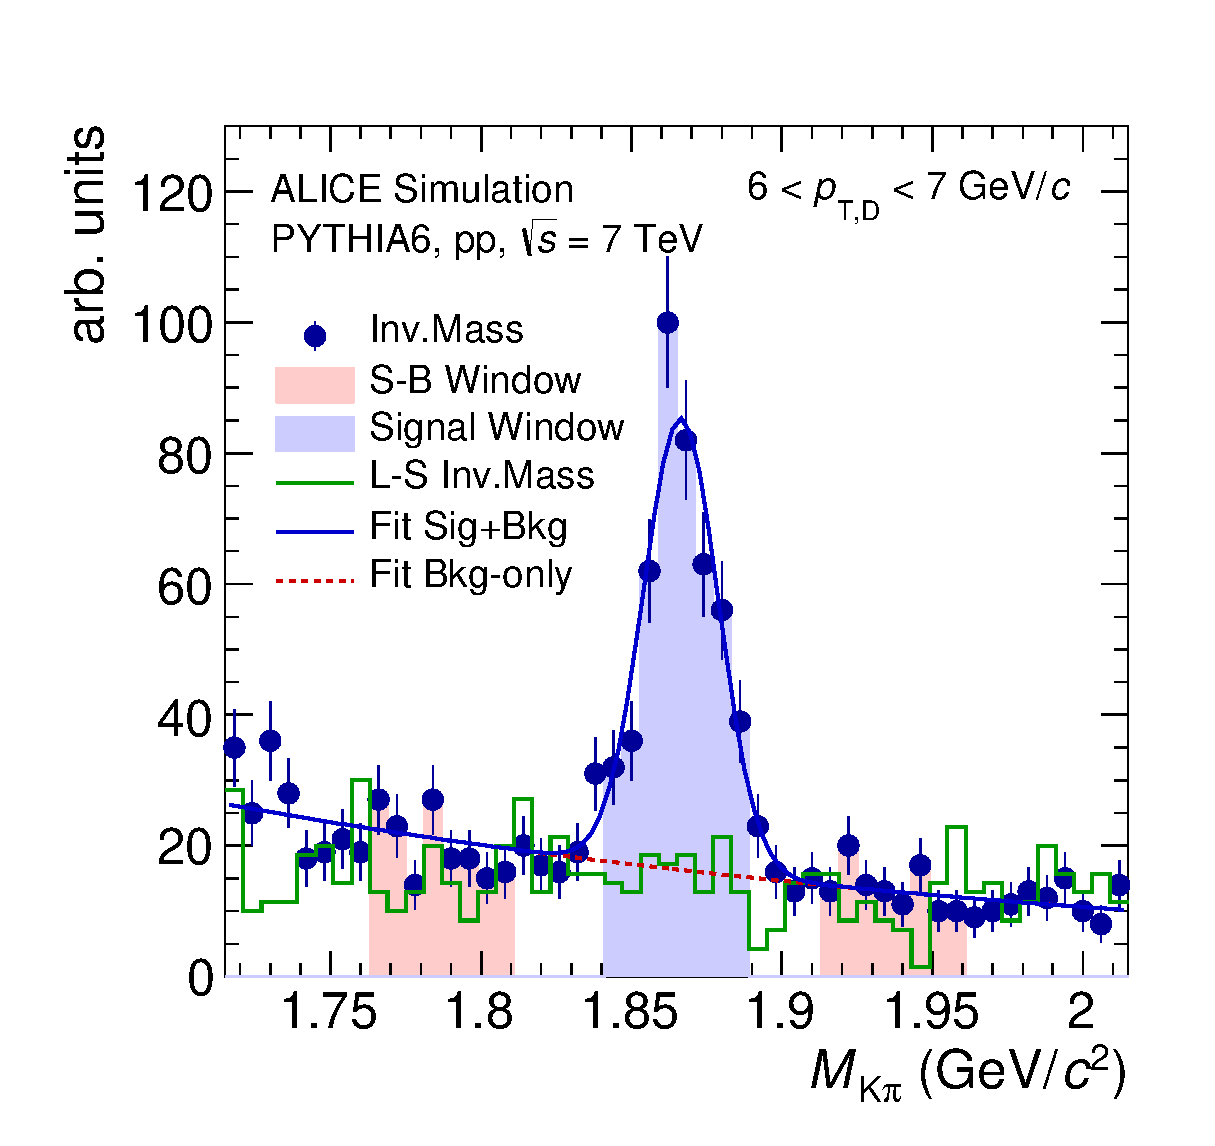
\includegraphics[width=0.8\textwidth]{img/HQ16_Simulation_InvMassSB}
 \caption{Invariant mass distribution for $6 < \ptd < 7$~\GeVc; the plot shows also the signal region, the S-B regions and the L-S invariant mass; the fit curves are show as well.} 
 \label{fig:HQ16_Simulation_InvMassSB}
\end{center}
\end{figure}
Figure~\ref{fig:HQ16_Simulation_InvMassSB} shows the invariant mass distribution for $6 < \ptd < 7$~\GeVc. 

The signal extraction is validated by comparing the spectra obtained with the three methods outlined above with the MC truth. 
\begin{figure}[tbh]
\centering
\begin{subfigure}{0.49\textwidth}
  \centering
  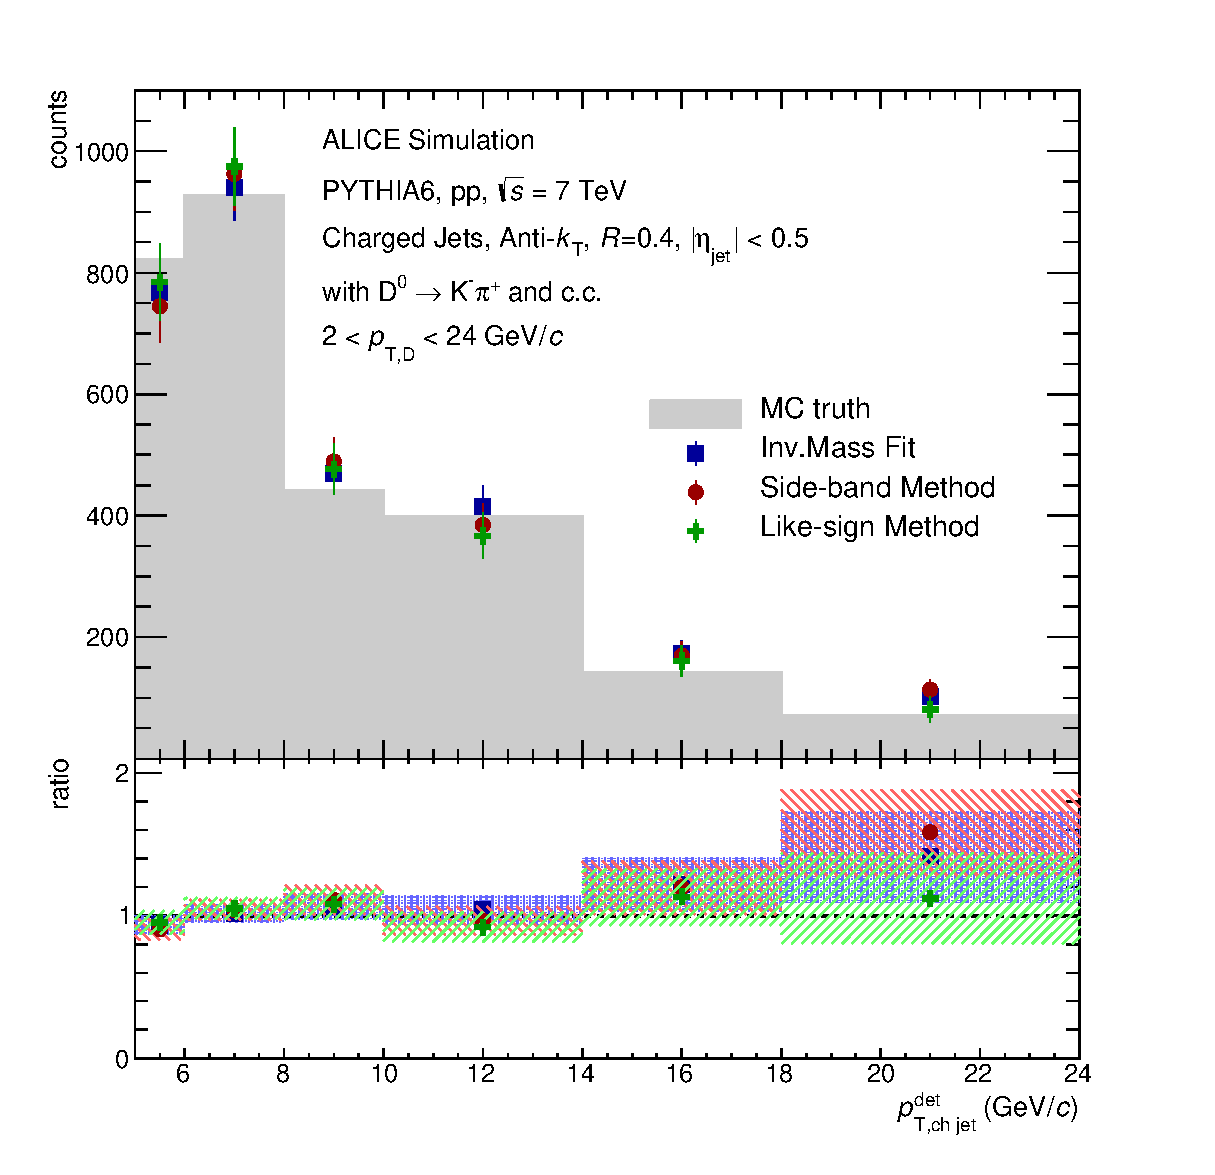
\includegraphics[width=1.0\linewidth]{img/HQ16_Simulation_MethodComparison}
  \caption{Yields.}
  \label{fig:HQ16_Simulation_MethodComparison}
\end{subfigure}
\begin{subfigure}{0.49\textwidth}
  \centering
  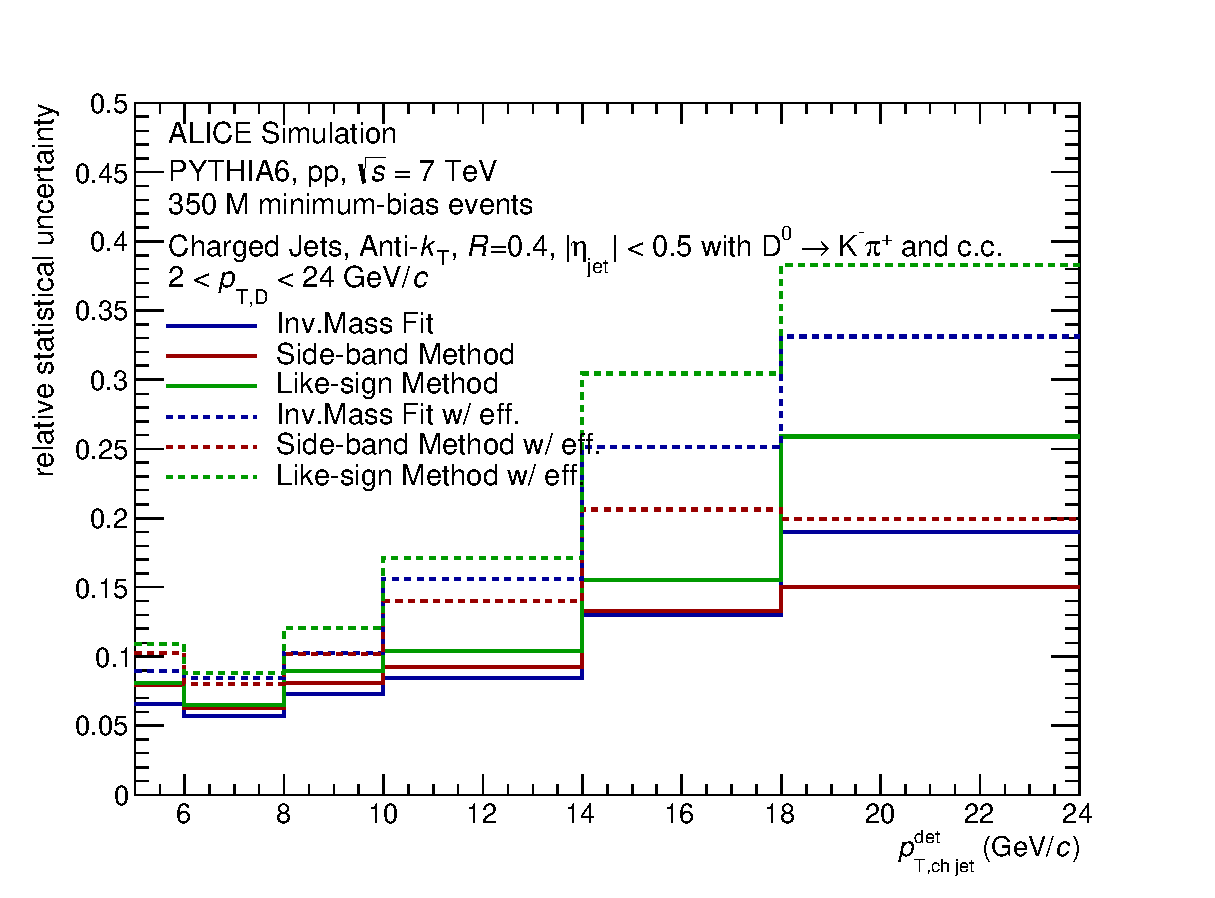
\includegraphics[width=1.0\linewidth]{img/HQ16_Simulation_UncertaintyComparison}
  \caption{Statistical uncertainties.}
  \label{fig:HQ16_Simulation_UncertaintyComparison}
\end{subfigure}
\caption{Comparison of the invariant mass fit, L-S and S-B methods.}
\label{fig:MethComp}
\end{figure}
The invariant mass fit, L-S and S-B methods all show good performances in recovering the signal, as shown in Fig.~\ref{fig:HQ16_Simulation_MethodComparison}.
In Fig.~\ref{fig:HQ16_Simulation_UncertaintyComparison} the statistical precisions achieved by each method are compared. The statistical uncertainties are
also shown for spectra corrected for the reconstruction efficiency. The statistical uncertainties are affected because efficiency correction alters the 
relative contribution of \Dzero\ mesons with different \pt\ in each \ptchjet\ bin.
%%%%%%%%%%%%
%%%%%%%%%%%%
\section{Work In Progress figure}
Figure~\ref{fig:HQ16_WorkInProgress_StatisticalUncertainty} is a work-in-progress plot that shows the statistical uncertainty of the D-tagged jets in all the available data for \pp\ collisions at \s~$=7$~TeV collected in 2010.
This corresponds to about 300 M minimum bias events. The signal is extracted via an invariant mass fit in jet \pt\ bins.
\begin{figure}[tbh]
\begin{center}
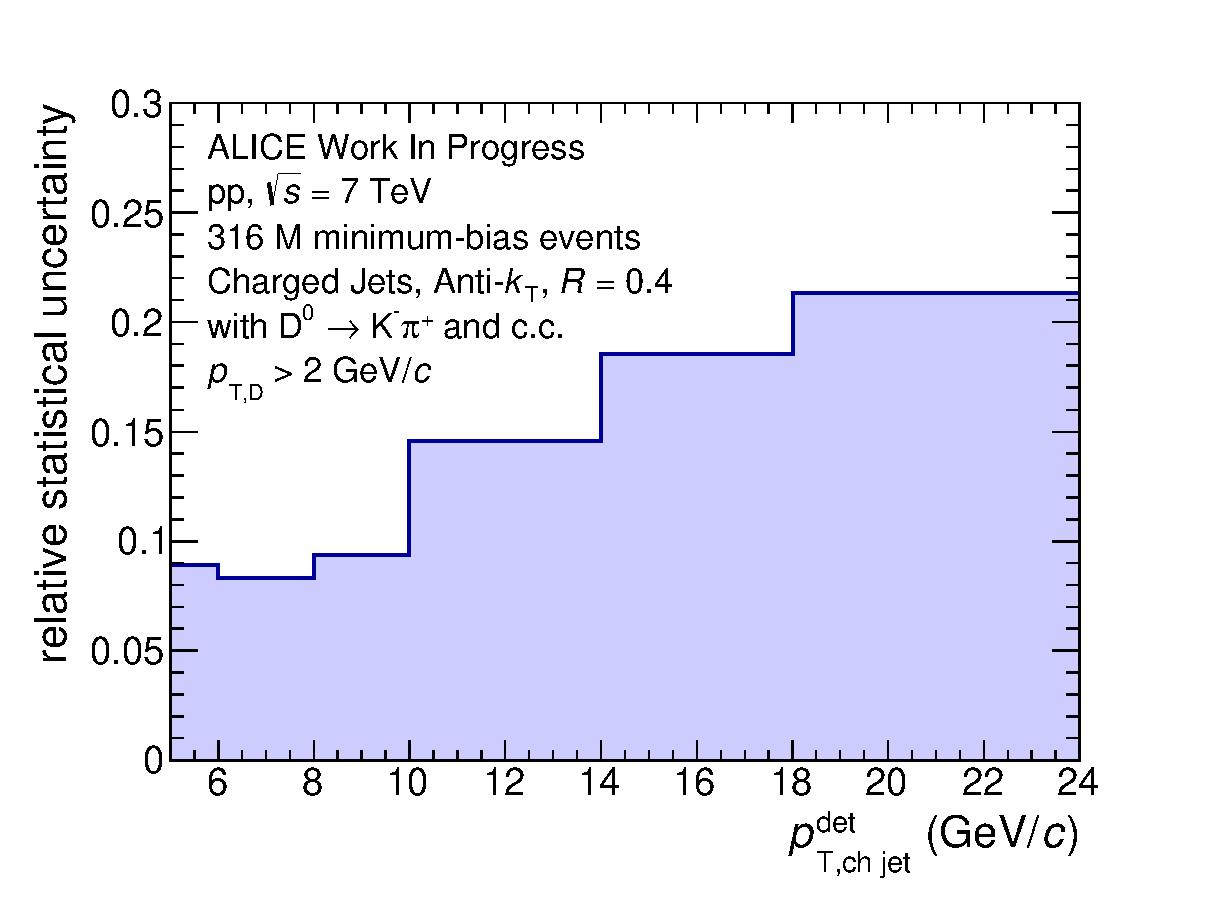
\includegraphics[width=0.8\textwidth]{img/HQ16_WorkInProgress_StatisticalUncertainty}
 \caption{Relative statistical uncertainty for D-tagged jets in 2010 pp data.} 
 \label{fig:HQ16_WorkInProgress_StatisticalUncertainty}
\end{center}
\end{figure}
%%%%%%%%%%%%